\chapter{Aspectos Conceituais}
\section{Levantamento de Requisitos}
Em Engenharia de Software, é essencial o momento do levantamento de requisitos, dado que são eles que ditam o funcionamento do software a ser desenvolvido, alinha as expectativas dos \textit{stakeholders} e determinam os requisitos funcionais e não funcionais necessários para a aceitação. Neste projeto, para o levantamento de requisitos, foi usada uma das técnicas descritas em \cite{kurtbittnerianspence2002}, que consiste em levantar primeiramente os \textit{stakeholders} do projeto. Segundo \cite{kurtbittnerianspence2002}, a definição traduzida de \textit{stakeholder} é a seguinte:

\begin{citacaoLonga}
"Um indivíduo que é materialmente afetado pelo resultado do
sistema ou o(s) projeto(s) que produzem o sistema."
\end{citacaoLonga}

Ou seja, \textit{stakeholders} não são apenas os indivíduos que efetivamente usarão o sistema, mas sim todos os impactados sua existência. O livro divide os \textit{stakeholders} em 5 grupos:

\begin{itemize}
    \item Usuários: as pessoas que efetivamente usarão o sistema.
    \item Patrocinadores: os financiadores do projeto de software que gerará o sistema.
    \item Desenvolvedores: os responsáveis por desenvolver o sistema levantado pelo processo.
    \item Autoridades: órgãos reguladores que determinam regras para o uso de determinado software.
    \item Consumidores: empresas que compram esses softwares para serem usados.
\end{itemize}

\subsection{Entendimento dos Problemas}

Uma vez mapeado os \textit{stakeholders}, partimos para entender agora as dores que cada um possui e o que eles esperam com o produto final a ser desenvolvido. Alguns processos são sugeridos pelo livro\cite{kurtbittnerianspence2002}, como por exemplo:

\begin{itemize}
    \item Entrevistas: entrevistar os envolvidos e entender diretamente quais são suas dores e expectativas.
    \item Questionários: São úteis quando há um amplo número de \textit{stakeholders} envolvidos.
    \item Grupo Focal: Reunião com alguns representantes dos grupos de \textit{stakeholders} para entender e construir uma visão única sobre o projeto.
    \item Quadros de Aviso: É um tipo particular de grupo focal, onde o quadro serve como unificador da visão, com a diferença de não ter todos reunidos ao mesmo tempo.
    \item \textit{Workshops}: Eventos avisados com antecedência para entender melhor sobre o sistema, com a participação dos envolvidos.
    \item Revisões: Reuniões informais com o intuito de revisar documentos gerados com alguns envolvidos.
    \item Encenação: É uma técnica facilitadora usada em conjunto com \textit{workshops} para obter informações mais específicas ou \textit{feedbacks}.
\end{itemize}

Com essa listagem de problemas levantados pelos processos de levantamento de requisitos, finalmente podemos partir para a visão unificada do processo como um todo e como o software vai atuar no processo. Para isso, é saudável a elaboração de um documento unificando os pontos de vista dos \textit{stakeholders} e estabelecendo o que de fato será o sistema a ser desenvolvido, resultando no Documento de Visão.

\subsection{Documento de Visão}

O documento de visão, segundo o livro\cite{kurtbittnerianspence2002}, traz a seguinte definição (traduzida):

\begin{citacaoLonga}
O Documento de Visão é o artefato do Rational Unified Process\cite{ibm2011} que capta todas as informações de requisitos. Como toda documentação de requisitos, seu objetivo principal é a comunicação.
\end{citacaoLonga}

Existem diversos modelos de Documento de Visão, porém, em sua essência, atendem os seguintes tópicos\cite{kurtbittnerianspence2002}:

\begin{enumerate}
    \item Posicionamento: Como o sistema irá se posicionar no quesito de negócios? Há concorrentes que já resolvem o problema? Quais são seus diferenciais em relação a eles?
    \item \textit{Stakeholders} e usuários: Quem são os envolvidos direta e indiretamente com o desenvolvimento e a existência do sistema?
    \item Necessidades chave: Quais são as demandas que realmente precisam estar nos planos do sistema para satisfazer os envolvidos?
    \item Visão geral do produto: O que é o produto de fato? Quais são suas dependências, capacidades e alternativas ao seu desenvolvimento?
    \item Funcionalidades: Quais são as funcionalidades em alto nível do sistema, para que elas resolvam as necessidades chave listadas anteriormente?
    \item Outros requisitos do produto: Quais são os outros requisitos do sistema que não foram capturados como funcionalidades?
\end{enumerate}

\section{Histórias de Usuário}

Uma das abordagens possíveis para se estabelecer os requisitos levantados e começar a desenvolver de fato o sistema é o uso de Histórias de Usuários (ou \textit{User Stories}). A definição de Histórias de Usuário, traduzido de \cite{jonathanrasmusson}, está a seguir:

\begin{citacaoLonga}
São descrições curtas das funcionalidades que o nosso cliente
gostaria de um dia ver em seu software. Eles geralmente são escritos em pequenos cartões de índice (para nos lembrar de não tentar escrever tudo) e estão lá para nos encorajar a ir falar com nossos clientes.
\end{citacaoLonga}

\subsection{Escopo base da história}
O essencial em escrever boas histórias de usuário está em agregar valor para os \textit{stakeholders}. Ou seja, escrever histórias de usuário que tangem assuntos como arquitetura do sistema, linguagem de implementação, padrões de código entre outros não são boas histórias de usuário, pois salvo raríssimas exceções, o cliente não vê valor em histórias desse tipo.

Em contrapartida, histórias sobre o comportamento do sistema que carregam valor de produto nelas são histórias de usuário importantes para o processo de desenvolvimento. Muitas vezes, porém, histórias de usuário forçam um viés altamente técnico; nessas situações, cabe buscar a causa raiz que levou à "solução" escrita na história: histórias de usuário apresentam problemas de negócio, jamais soluções técnicas.

\subsection{Características básicas}

Boas histórias de usuário costumam ser independentes entre si. Tal independência é importantíssima para mudanças no projeto (que ocorrem com frequência), porque histórias isoladas são fáceis de serem alteradas. Outro ponto importante está em elas serem negociáveis, ou seja, elas podem sofrer alterações e inclusive serem removidas se, com o andamento do projeto, ela perder sua prioridade e tais alterações e remoções não afetam o andar geral das outras tarefas.

Por fim, elas precisam de mais duas características fundamentais: precisam ser testáveis (e quantificar esses testes, se possível), tanto no fluxo de negócio como na escrita de testes automatizados, assim podemos garantir com facilidade a qualidade do que está sendo entregue e; precisam ser pequenas e estimáveis, ou seja, o esforço dela pode ser previsto com antecedência (essa por projetos anteriores ou pela experiência dos integrantes da equipe), permitindo assim medidas de performance dos envolvidos, escopo entregue, entre outros.

\subsection{Um padrão para Histórias de Usuário}

Um bom padrão para escrever histórias de usuário está a seguir\cite{jonathanrasmusson}:

\begin{citacaoLonga}
Eu como $<$para quem é a história$>$
\\
Eu quero $<$o que ele quer$>$
\\
por causa $<$por que ele quer$>$
\end{citacaoLonga}

\section{Casos de Uso}

Como outra alternativa para documentar o que será desenvolvido no sistema, há a solução clássica de desenvolvimento de software: casos de uso. Essencialmente, cada caso de uso possui um ou mais atores agindo com o sistema. Segundo as definições traduzidas de \cite{kurtbittnerianspence2002}:

\begin{citacaoLonga}
\textbf{Atores} representam as pessoas ou coisas que interagem de alguma forma com o sistema; por definição, eles estão fora do sistema. Eles têm um nome e uma breve descrição, e eles estão associados com os casos de uso com os quais eles interagem.
\\
\\
\textbf{Casos de Uso} representam as coisas de valor que o sistema executa para os atores. Casos de uso não são funções ou recursos e não podem ser decompostos. Casos de uso têm um nome e uma breve descrição. Eles também tem descrições detalhadas que são essencialmente histórias sobre como o atores usam o sistema para fazer algo que considerem importante, e que o sistema faz para satisfazer essas necessidades.
\end{citacaoLonga}

\subsection{Características básicas}
Casos de uso, como escrito acima, descrevem as interações entre os atores e o sistema projetado, logo, é coerente que eles estejam relacionados à um processo completo, com começo, meio e fim. Uma grande vantagem de uso dessa técnica está em estabelecer uma espécie de contrato entre a equipe de concepção do sistema e os \textit{stakeholders}, o que evita a participação constante dos envolvidos durante o desenvolvimento.

Um fator interessante está na concepção do documento dos casos de uso, pois ela pode ocorrer de duas formas: como um documento resultante do documento de visão, gerado durante o levantamento de requisitos, ou como uma estratégia para levantar os requisitos e, como consequência, gerar o documento de visão\cite{elisayuminakagawa2013}.

\subsection{Uma estrutura de caso de uso}
Essencialmente, um caso de uso deve possuir a seguinte estrutura\cite{funpar2001}, baseada em \cite{ibm2011}:

\begin{enumerate}
    \item Nome: Nome do Caso de Uso
    \begin{enumerate}
        \item Breve Descrição: Finalidade do caso de uso
    \end{enumerate}
    \item Fluxo de Eventos: A descrição dos eventos que ocorrem no sistema, que são divididos em dois conjuntos principais.
    \begin{enumerate}
        \item Fluxo Básico: É o comportamento básico da interação entre os atores e o sistema. Aqui não devemos ter situações de contorno nem exceções, isso fica ao encargo dos fluxos alternativos.
        \item Fluxos Alternativos: Comportamentos diferenciados do caso de uso, podendo haver mais de um.
    \end{enumerate}
    \item Requisitos Especiais: Requisito não funcional que é específico de um caso de uso, mas que não está contemplado no fluxo de eventos.
    \item Pré-condição: Estado do sistema antes da realização do caso de uso.
    \item Pós-condição: Possíveis estados do sistema após a execução do caso de uso.
\end{enumerate}

Essa estrutura é interessante, pois atende o que deve ser um caso de uso: deve fugir de uma estrutura pequena, englobando um fluxo bem definido do sistema e que traga valor de negócio para os envolvidos. Além disso, com sua descrição comportamental, ele serve como um contrato estabelecido de desenvolvimento, o que abona a participação integral dos \textit{stakeholders}, como é de se esperar de um caso de uso.

\section{Verificação e Validação}

Durante o desenvolvimento, é saudável garantir a qualidade do que está sendo entregue, tanto na parte técnica, quanto no alinhamento com a parte de negócios do projeto. Para isso, existem os processos de verificação e validação, traduzidos do SWEBOK\cite{ieeecomputersociety2014}:

\begin{citacaoLonga}
O objetivo da verificação e validação é ajudar a equipe de desenvolvimento a garantir qualidade no sistema por todo seu ciclo de vida.
\end{citacaoLonga}

\subsection{Verificação}
Em desenvolvimento de software, é uma boa prática acompanhar se os requisitos funcionais e não funcionais estão sendo atendidos, de preferência com acompanhamento das métricas determinadas nos requisitos. Essa prática é conhecida como verificação, definida de maneira resumida pela seguinte pergunta\cite{eduardofigueiredo2018}:

\begin{citacaoLonga}
Estamos construindo o produto corretamente?
\end{citacaoLonga}

\subsection{Validação}
Além de acompanhar os requisitos propostos, é importante entender se o sistema está de acordo com as expectativas operacionais dos \textit{stakeholders}. Essa análise constante de adequação voltada aos negócios é conhecida como validação, definida pela seguinte questão\cite{eduardofigueiredo2018}:

\begin{citacaoLonga}
Estamos construindo o produto correto?
\end{citacaoLonga}

\subsection{Testes}
Em ambos os casos descritos acima, é necessário ter uma ferramenta que automatize esses processos e permita manter a consistência do que foi entregue quando há novas funcionalidades a serem lançadas. Para isso, existe o conceito de testes, onde o sistema passa por uma bateria de exames e revisões para detectar erros e garantir a qualidade e alinhamento do que foi entregue. Vale lembrar que essa bateria de testes é finita, sendo um subgrupo dos infinitos fluxos de execução do domínio\cite{ieeecomputersociety2014}.

Na escala macroscópica, temos os testes de aceitação junto aos \textit{stakeholders}, para validar a conformidade dos requisitos e a qualidade das entregas. Já para testar a arquitetura, costumam ser realizados testes de sistema. Para testar os componentes desenvolvidos do sistema, realizam-se testes de integração entre esses componentes. E, por fim, o código escrito para cada componente elaborado é testado pelos testes de unidade.

\begin{figure}[H]
    \centering
    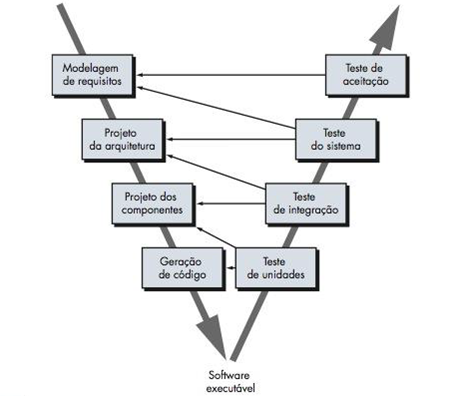
\includegraphics[scale=0.90]{modelo-v.png}
    \caption{Estrutura de Testes Modelo V\cite{devmedia2013}}
    \label{fig:modelo-v}
\end{figure}

Ao desenvolver um sistema, cada teste deve ser executado a cada nova funcionalidade adicionada e/ou modificada, pois só assim é possível garantir a qualidade do que já foi entregue. Uma boa prática para realizar esses testes, em especial os testes menores, é automatizar a execução deles, o que economiza tempo de uma pessoa dedicada à função de testador.
